%
% budgets.tex
%
% Copyright (C) 2021 by SpaceLab.
%
% GOLDS-UFSC Documentation
%
% This work is licensed under the Creative Commons Attribution-ShareAlike 4.0
% International License. To view a copy of this license,
% visit http://creativecommons.org/licenses/by-sa/4.0/.
%

%
% \brief Budgets and mission analysis chapter.
%
% \author Gabriel Mariano Marcelino <gabriel.mm8@gmail.com>
%
% \institution Universidade Federal de Santa Catarina (UFSC)
%
% \version 0.2.0
%
% \date 2020/06/11
%

\chapter{Technical Budgets and Mission Analysis} \label{ch:budgets}

This chapter presents a general analysis of the mission, such as a preliminary analysis of the satellite's estimated orbit, estimated lifetime, and the amount of data exchanged along its operation.

Another type of analysis presented is the satellite budgets, such as the power and link budgets.

\section{Requirements}

This section describes the operational and functional technical requirements for the Space System Catarina-A1. Applicable documents that justify the requirements presented in this document are the \ac{MDD} \cite{MDD} and the \ac{MA} \cite{MA}.

The Mission Requirements and the System Requirements are presented according to the following nomenclature:

\begin{itemize}
    \item REQ-MIS: Mission Requirements;
    \item REQ-CDS: CubeSat Design Specification Requirements;
    \item REQ-PAY: Primary Payload System Requirements;
    \item REQ-SER: Service System Requirement.
\end{itemize}

This document is based on the ECSS-E-ST-10-06C \cite{ECSS-E-ST-10C} standard (specifically using the template presented in Annex A). However, information about the user’s needs, mission goals and objectives, and mission conception are presented in \cite{MDD}.

\subsection{Mission requirements}

The Mission Requirements are displayed in \autoref{tab:mission-requirements}, which presents its ID, approval date, and revision date. The respective rationale, traceability, and verification method can be found in the Requirement Justification Files \cite{RJF_A1} \cite{RJF_A2}.

\begin{table}[H] \footnotesize
    \centering
    \begin{tabular}{p{1.9cm}p{6cm}p{3.8cm}p{2.8cm}}
        \toprule[1.5pt]
        \textbf{ID} & \textbf{Description} & \textbf{Initial Approval Date} & \textbf{Revision Date} \\
        \midrule
        REQ-MIS-1 & Catarina Constellation - Fleet A   must collect data transmitted by Data Collection Platforms & 25/02/2022–Delta-\acs{MDR} & 04/08/2022 - \acs{SRR} \\
        REQ-MIS-2 & The Space Segment from Catarina Constellation - Fleet A  must send the collected data to the \ac{EMMN} & 25/02/2022–Delta-\acs{MDR} & 04/08/2022 - \acs{SRR} \\
        REQ-MIS-3 & The \ac{EMMN} must control the Space Segment of Catarina Constellation - Fleet A & 25/02/2022–Delta-\acs{MDR} & 04/08/2022 - \acs{SRR} \\
        REQ-MIS-4 & \ac{SINDA} must be used to distribute the collected data by the Space Segment & 25/02/2022–Delta-\acs{MDR} & 04/08/2022 - \acs{SRR} \\
        REQ-MIS-5 & The linkage \ac{DCP}-Space Segment must be able to receive not less than   32 bytes per access. & 25/02/2022–Delta-\acs{MDR} & 04/08/2022 - \acs{SRR} \\
        REQ-MIS-6 & The linkage of Data Collection must be compatible with \ac{ARGOS} protocol & 25/02/2022–Delta-\acs{MDR} & 04/08/2022 - \acs{SRR} \\
        REQ-MIS-8 & The linkage \ac{EMMN}-Space Segment must be able to transport not less than 32 bytes per access. & 25/02/2022–Delta-\acs{MDR} & 04/08/2022 - \acs{SRR} \\
        REQ-MIS-9 & The mission data must be compatible with the data structure defined   by the \ac{SBCD} & 25/02/2022–Delta-\acs{MDR} & 04/08/2022 - \acs{SRR} \\
        REQ-MIS-10 & Two CubeSats must be successfully designed and integrated by the team & 04/08/2022 - \acs{SRR} & 04/08/2022 - \acs{SRR} RID \\
        REQ-MIS-11 & The CubeSats must be able of operating in LEO at an altitude between   500 and 650 km and inclination between 20 to 100 degrees & 04/08/2022 - \acs{SRR} & 04/08/2022 - \acs{SRR} \\
        \bottomrule[1.5pt]
    \end{tabular}
    \caption{Mission Requirements for Catarina Constellation - Fleet A.}
    \label{tab:mission-requirements}
\end{table}

\subsection{System requirements}

The system requirements are divided by Space Segment into two documents. The system requirements applicable for the Catarina-A1 Space System are described herein. The system requirements applicable for the Catarina-A2 Space System are described in \cite{TRJ_A2}. System requirements applicable to the Ground Segment are identical for both space systems and, for such, are presented in both documents. 

The System Requirements defined are indicated in the subsections below, divided into three sections: CubeSat Design Specification Requirements, Primary Payload System Requirements, and Service System Requirements. The respective rationale, traceability, and verification method can be found in the Requirement Justification File \cite{RJF_A1}.

\subsubsection{CubeSat Design Specification Requirements} \label{sec:cubesat_requirements}

The requirements described in the CubeSat Design Specification \cite{Cubesat_Specification}, applicable for a 2U CubeSat, are indicated in \autoref{cubesat_requirementsA}. At this mission stage, the Launch Provider is not yet defined. To pursue compliance with most of the possible Launch Provider requirements, the CubeSat Design Specification requirements are herein defined as part of the System Requirements for this mission. All references in \autoref{cubesat_requirementsA} to \autoref{cubesat_requirementsE} are related to \cite{Cubesat_Specification}.

\begin{table}[H] \footnotesize
    \centering
    \begin{tabular}{p{2cm}p{8.5cm}p{3cm}}
        \toprule[1.5pt]
        \textbf{ID} & \textbf{Description} & \textbf{Initial Approval Date} \\
        \midrule
        REQ-CDS-1 & All parts shall remain attached to the CubeSats during launch, ejection and operation & 10/03/2023 - \acs{SRR} RID \\
        REQ-CDS-2 & Pyrotechnics shall conform to AFSPCMAN 91-710, Volume 3. & 10/03/2023 - \acs{SRR} RID \\
        REQ-CDS-3 & Any propulsion systems shall be designed, integrated, and tested in accordance with AFSPCMAN 91-710 Volume 3 & 10/03/2023 - \acs{SRR} RID \\
        REQ-CDS-4 & Propulsion systems shall have at least 3 inhibits to activation. & 10/03/2023 - \acs{SRR} RID \\
        REQ-CDS-5 & CubeSat hazardous materials shall conform to AFSPCMAN 91-710, Volume 3. & 10/03/2023 - \acs{SRR} RID \\
        REQ-CDS-6 & CubeSat materials shall satisfy low out-gassing criteria, as defined in 2.1.7.1 and 2.1.7.2,
        to prevent contamination of other spacecraft during integration, testing, and launch. A list
        of NASA approved low out-gassing materials can be found at: http://outgassing.nasa.gov &  10/03/2023 - \acs{SRR} RID \\
        REQ-CDS-7 & CubeSats materials shall have a Total Mass Loss (TML) of less than or equal to 1.0 \% & 10/03/2023 - \acs{SRR} RID \\
        REQ-CDS-8 & CubeSat materials shall have a Collected Volatile Condensable Material (CVCM) of
        less than or equal to 0.1\% & 10/03/2023 - \acs{SRR} RID \\
        REQ-CDS-9 & The magnetic field of any passive magnets shall be limited to 0.5 Gauss above Earth’s
        magnetic field, outside the CubeSat static envelope. & 10/03/2023 - \acs{SRR} RID \\
        REQ-CDS-10 & The CubeSat shall be designed to accommodate ascent venting per ventable volume/area
        of less than 50.8 meters (2000 inches). & 10/03/2023 - \acs{SRR} RID \\
        REQ-CDS-11 & The CubeSat shall use the coordinate system as defined in Appendix B. The origin of the
        CubeSat coordinate system is located at the geometric center of the CubeSat. & 10/03/2023 - \acs{SRR} RID \\
        REQ-CDS-12 & The CubeSat configuration and physical dimensions shall conform to the appropriate
        section of Appendix B. & 10/03/2023 - \acs{SRR} RID \\
        REQ-CDS-13 & The –Z face of the CubeSat will be inserted first into the dispenser & 10/03/2023 - \acs{SRR} RID \\
        REQ-CDS-14 & No components on the yellow shaded sides (see Appendix B CDS drawings) shall protrude
        farther than 6.5 mm normal to the surface from the plane of the rail & 10/03/2023 - \acs{SRR} RID \\
        REQ-CDS-15 & Deployables shall be constrained by the CubeSat, not the dispenser. This requirement
        originates from requirements of most Launch Providers. & 10/03/2023 - \acs{SRR} RID \\
        REQ-CDS-16 & Rails should have a surface roughness less than 1.6 µm. & 10/03/2023 - \acs{SRR} RID \\
        \bottomrule[1.5pt]
    \end{tabular}
    \caption{CubeSat Design Specification Requirements for Catarina-A1 (Part A).}
    \label{cubesat_requirementsA}
\end{table}

\begin{table}[H] \footnotesize
    \centering
    \begin{tabular}{p{2cm}p{8.5cm}p{3cm}}
        \toprule[1.5pt]
        \textbf{ID} & \textbf{Description} & \textbf{Initial Approval Date} \\
        \midrule
        REQ-CDS-17 & The 1U, 1.5U, and 2U CubeSat separation spring must be centered on the end of the standoff on the CubeSat’s –Z face as per Figure 7. & 10/03/2023 - \acs{SRR} RID \\
        REQ-CDS-18 & At least 75\% of the rail should be in contact with the dispenser rails. 25\% of the rails may be recessed. & 10/03/2023 - \acs{SRR} RID \\
        REQ-CDS-19 & The CubeSat center of gravity shall fall within the ranges specified in Table 2 & 10/03/2023 - \acs{SRR} RID \\
        REQ-CDS-20 & The CubeSat structure should be made from aluminum alloy. Note: Typically, Aluminum 7075, 6061, 6082, 5005, and/or 5052 are used for both the main CubeSat structure and the rails. If materials other than aluminum are used, the CubeSat developer should contact the Launch Provider or dispenser manufacturer. & 10/03/2023 - \acs{SRR} RID \\
        REQ-CDS-21 & Any aluminum CubeSat external surfaces, such as rails and standoffs that are in contact with the dispenser rails, shall be hard anodized to prevent any cold welding within the dispenser. & 10/03/2023 - \acs{SRR} RID \\
        REQ-CDS-22 & If a CubeSat shares a dispenser with another CubeSat(s), each CubeSat shall employ a mechanism to encourage separation from neighboring CubeSats within the dispenser. & 10/03/2023 - \acs{SRR} RID \\
        REQ-CDS-23 &  The separation mechanism shall not extend beyond the level of the standoff in a
        stowed configuration. & 10/03/2023 - \acs{SRR} RID \\
        REQ-CDS-24 &  To prevent CubeSat from activating any powered functions, the CubeSat power system shall be at a power-off state from the time of delivery to the LV through on-orbit deployment & 10/03/2023 - \acs{SRR} RID \\
        REQ-CDS-25 &  The CubeSat shall have, at a minimum, one deployment switch, which is actuated while integrated in the dispenser. & 10/03/2023 - \acs{SRR} RID \\
        REQ-CDS-26 & In the actuated state, the CubeSat deployment switch shall electrically disconnect the power system from the powered functions. & 10/03/2023 - \acs{SRR} RID \\
        REQ-CDS-27 &  The deployment switch shall be in the actuated state at all times while integrated in the dispenser. & 10/03/2023 - \acs{SRR} RID \\
        REQ-CDS-28 &  In the actuated state, the CubeSat deployment switch should be at or below the level of any external surface that interfaces with the dispenser or neighboring CubeSat. This ensures that the switch will not damage or interfere with the contacting surface. & 10/03/2023 - \acs{SRR} RID \\
        REQ-CDS-29 &  If the CubeSat deployment switch toggles from the actuated state and back, the satellite shall reset to a pre-launch state, including reset of transmission and deployable timers. & 10/03/2023 - \acs{SRR} RID \\
        \bottomrule[1.5pt]
    \end{tabular}
    \caption{CubeSat Design Specification Requirements for Catarina-A1 (Part B).}
    \label{cubesat_requirementsB}
\end{table}

\begin{table}[H] \footnotesize
    \centering
    \begin{tabular}{p{2cm}p{8.5cm}p{3cm}}
        \toprule[1.5pt]
        \textbf{ID} & \textbf{Description} & \textbf{Initial Approval Date} \\
        \midrule
        REQ-CDS-30 &  Real Time Clocks (RTC) may be permitted, if they satisfy requirements REQ-CDS-29 through REQ-CDS-31. & 10/03/2023 - \acs{SRR} RID \\
        REQ-CDS-31 &  RTC circuits shall be isolated from the CubeSat’s main power system. & 10/03/2023 - \acs{SRR} RID \\
        REQ-CDS-32 &  RTC frequencies shall be less than 320 kHz. & 10/03/2023 - \acs{SRR} RID \\
        REQ-CDS-33 &  RTC circuits shall be current limited to less than 10 mA. & 10/03/2023 - \acs{SRR} RID \\
        REQ-CDS-34 &  The RBF pin and all CubeSat umbilical connectors shall be within the designated access port locations if available on the CubeSat’s dispenser. Please contact the manufacturer for specific charging and diagnostic port locations and procedures. & 10/03/2023 - \acs{SRR} RID \\
        REQ-CDS-35 &  The CubeSat shall include an RBF pin, which cuts all power to the satellite once it is inserted into the satellite. & 10/03/2023 - \acs{SRR} RID \\
        REQ-CDS-36 &  Access to the CubeSat is not guaranteed during or after integration. The RBF pin shall be removed from the CubeSat before integration into the dispenser, if the dispenser does not have access ports. & 10/03/2023 - \acs{SRR} RID \\
        REQ-CDS-37 &  The RBF pin shall protrude no more than 6.5 mm from the CubeSat rail surface when it is fully inserted into the satellite & 10/03/2023 - \acs{SRR} RID \\
        REQ-CDS-38 &  CubeSats shall incorporate battery circuit protection for charging/discharging to avoid unbalanced cell conditions. Additional manufacturer documentation and/or testing will be required for modified, customized, or non-UL-listed cells. & 10/03/2023 - \acs{SRR} RID \\
        REQ-CDS-39 &  The CubeSat shall have at least three independent RF inhibits to prohibit inadvertent RF transmission. & 10/03/2023 - \acs{SRR} RID \\
        REQ-CDS-40 &  The CubeSat shall have at least three independent inhibits to prohibit the inadvertent release of any deployable structures such as antennas or solar panels. & 10/03/2023 - \acs{SRR} RID \\
        REQ-CDS-41 &  The CubeSat shall have at least three independent RF inhibits to prohibit inadvertent RF transmission. & 10/03/2023 - \acs{SRR} RID \\
        REQ-CDS-42 &  CubeSats shall comply with their country’s radio license agreements and restrictions. & 10/03/2023 - \acs{SRR} RID \\
        REQ-CDS-43 &  CubeSat mission design and hardware shall be in accordance with NPR 8715.6 to limit orbital debris & 10/03/2023 - \acs{SRR} RID \\
        REQ-CDS-44 &  Any CubeSat component shall re-enter with energy less than 15 Joules & 10/03/2023 - \acs{SRR} RID \\
        REQ-CDS-45 &  Developers should be ready to provide orbital debris mitigation data if requested by the licensing agency or Launch Provider. & 10/03/2023 - \acs{SRR} RID \\
    \end{tabular}
    \caption{CubeSat Design Specification Requirements for Catarina-A1 (Part C).}
    \label{cubesat_requirementsC}
\end{table}

\begin{table}[H] \footnotesize
    \centering
    \begin{tabular}{p{2cm}p{8.5cm}p{3cm}}
        \toprule[1.5pt]
        \textbf{ID} & \textbf{Description} & \textbf{Initial Approval Date} \\
        \midrule
        REQ-CDS-46 &  All deployables such as booms, antennas, and solar panels shall wait to deploy a minimum of 30 minutes after the CubeSat's deployment switch(es) are activated during dispenser ejection & 10/03/2023 - \acs{SRR} RID \\
        REQ-CDS-47 &  CubeSats shall not generate or transmit a signal earlier than 45 minutes after on-orbit deployment. & 10/03/2023 - \acs{SRR} RID \\
        REQ-CDS-48 &  The dispenser developer will conduct a minimum of one fit check in which the CubeSat flight unit will be inspected and integrated into the dispenser or engineering dispenser to verify the fit. A final fit check will be conducted just prior to integration of the CubeSat flight unit to the dispenser. & 10/03/2023 - \acs{SRR} RID \\
        REQ-CDS-49 &  Random vibration testing shall be performed to the levels and duration as defined by the Launch Provider. & 10/03/2023 - \acs{SRR} RID \\
        REQ-CDS-50 &  Thermal vacuum bakeout shall be performed to ensure proper outgassing of components. & 10/03/2023 - \acs{SRR} RID \\
        REQ-CDS-51 &  Shock testing must be performed as defined by the launch provider. & 10/03/2023 - \acs{SRR} RID \\
        REQ-CDS-52 &  Visual inspection of the CubeSat and measurement of critical areas will be performed per the CIFP (cubesat.org) or as defined by the Launch Provider. & 10/03/2023 - \acs{SRR} RID \\
        REQ-CDS-53 & Qualification testing is performed on an engineering unit that is identical to the flight model CubeSat. Qualification levels will be determined by the Launch Provider. Both SMC-S-016 and GSFC-STD-7000A are used as guides in determining test levels and durations. The flight model will then be tested to acceptance levels on its own. The Launch Provider may also require a final acceptance/workmanship random vibration test on the CubeSat and flight dispenser after integration & 10/03/2023 - \acs{SRR} RID \\
        REQ-CDS-54 & Protoflight testing is performed on the flight model CubeSat. Protoflight levels will be determined by the Launch Provider. Both SMC-S-016 and GSFC-STD-7000A are used as guides in determining test levels and durations. The flight model will be tested to protoflight levels on its own. The Launch Provider may also require a final acceptance/workmanship random vibration test on the CubeSat and flight dispenser after integration. The flight CubeSat shall not be disassembled or modified after protoflight testing. Disassembly of hardware after protoflight testing will require the developer to adhere to the waiver process prior to disassembly & 10/03/2023 - \acs{SRR} RID \\
        \bottomrule[1.5pt]
    \end{tabular}
    \caption{CubeSat Design Specification Requirements for Catarina-A1 (Part D).}
    \label{cubesat_requirementsD}
\end{table}

\begin{table}[H] \footnotesize
    \centering
    \begin{tabular}{p{2cm}p{8.5cm}p{3cm}}
        \toprule[1.5pt]
        \textbf{ID} & \textbf{Description} & \textbf{Initial Approval Date} \\
        \midrule
        REQ-CDS-55 & After delivery and integration of the CubeSat into the dispenser, additional testing may be performed on the integrated system. This test ensures proper integration of the CubeSat into the dispenser. Acceptance test levels will be determined by the Launch Provider. Both SMC-S-016 and GSFC-STD-7000A are used as guides in determining testing levels. The CubeSat shall not be deintegrated at this point. If a CubeSat failure is discovered, a decision to deintegrate the dispenser will be made by the Launch Provider based on mission safety concerns. & 10/03/2023 - \acs{SRR} RID \\
        \bottomrule[1.5pt]
    \end{tabular}
    \caption{CubeSat Design Specification Requirements for Catarina-A1 (Part E).}
    \label{cubesat_requirementsE}
\end{table}

\subsubsection{Primary Payload System Requirements} \label{sec:primary_payload_system_requirements}

The Primary Payload System Requirements for the Catarina-A1 are described in \autoref{primary_payload}. 

\begin{table}[H] \footnotesize
    \centering
    \begin{tabular}{p{2cm}p{8cm}p{3cm}}
        \toprule[1.5pt]
        \textbf{ID} & \textbf{Description} & \textbf{Initial Approval Date} \\
        \midrule
        REQ-PAY-01 & The primary payload shall be a communications system compatible with the \ac{DCP} & 04/08/2022 - \acs{SRR} \\
        REQ-PAY-02 & All data shall be capable of being traced to the date and time the data was taken & 04/08/2022 - \acs{SRR} \\
        REQ-PAY-03 & The primary payload shall be compatible with \ac{ARGOS}-2 protocol & 04/08/2022 - \acs{SRR} \\
        \bottomrule[1.5pt]
    \end{tabular}
    \caption{Primary Payload System Requirements for Catarina-A1.}
    \label{primary_payload}
\end{table}

\subsubsection{Service System Requirements} \label{sec:service_system_requirements}

The Service System Requirements for the Catarina-A1 are described in \autoref{service_system} and sub-divided into types, namely: functional, operational, interface, environmental, and design.  

\begin{table}[H] \footnotesize
    \centering
    \begin{tabular}{p{2cm}p{3cm}p{7.3cm}p{3cm}}
        \toprule[1.5pt]
        \textbf{ID} & \textbf{Type} & \textbf{Description} & \textbf{Initial Approval Date} \\
        \midrule
        REQ-SER-01 & Functional & The Catarina-A1 must receive, store and transmit collected data from data collection plataforms & 04/08/2022 - \acs{SRR} \\
        REQ-SER-02 & Operational & The target minimum operational service of the space system shall be 1 year, subjected to confirmation at \ac{CDR} & 04/08/2022 - \acs{SRR} \\
        REQ-SER-03 & Interface & The Catarina-A1 satellite shall dialogue with the ground segment using telemetry and telecommands & 04/08/2022 - \acs{SRR} \\
        REQ-SER-04 & Environmental & The antenna systems of the Catarina-A1 shall operate within the temperature range of -20 to 60 $^{\circ}$C & 04/08/2022 - \acs{SRR} \\
        REQ-SER-05 & Environmental & The solar panels module of the Catarina-A1 shall operate within the temperature range of -40 to 125 $^{\circ}$C & 04/08/2022 - \acs{SRR} \\
        REQ-SER-06 & Environmental & The \ac{EPS} module of the Catarina-A1 shall operate within the temperature range of -20 to 70 $^{\circ}$C & 04/08/2022 - \acs{SRR} \\
        REQ-SER-07 & Environmental & The \ac{OBDH} module of the Catarina-A1 shall operate within the temperature range of -25 to 65 $^{\circ}$C & 04/08/2022 - \acs{SRR} \\
        REQ-SER-08 & Environmental & The communication systems of the Catarina-A1 shall operate within the temperature range of -20 to 60 $^{\circ}$C & 04/08/2022 - \acs{SRR} \\
        REQ-SER-09 & Environmental & The structure of the Catarina-A1 shall operate within the temperature range of -40 to 80 $^{\circ}$C & 04/08/2022 - \acs{SRR} \\
        REQ-SER-10 & Operational & The satellite shall comply with the Brazil’s, ITU and IARU (for radioamateur) radio license agreements and   restrictions. & 04/08/2022 - \acs{SRR} \\
        REQ-SER-11 & Operational & The antenna systems of the Catarina-A1 shall be able to send signal at the frequency of TBC & 04/08/2022 - \acs{SRR} \\
        REQ-SER-12 & Operational & The antenna systems of the Catarina-A1 shall be able to receive signal at the frequency of TBC and 401,635 MHz & 04/08/2022 - \acs{SRR} \\
        REQ-SER-13 & Operational & The CubeSat shall be able to transmit not less than 32 bytes per access with the Ground Station & 04/08/2022 - \acs{SRR} \\
        REQ-SER-14 & Operational & The Catarina-A1 shall be able to store not less than 32 MB & 04/08/2022 - \acs{SRR} \\
        REQ-SER-15 & Operational & The Catarina-A1 shall have a mean of charging its battery that does not require   solar power & 04/08/2022 - \acs{SRR} \\
        REQ-SER-16 & Design - electrical & Following flight assembly, engineers should be able to examine the status of the Catarina-A1 via bus & 04/08/2022 - \acs{SRR} \\
        \bottomrule[1.5pt]
    \end{tabular}
    \caption{Service System Requirement for Catarina-A1.}
    \label{service_system}
\end{table}

\section{Orbit Parameters and Analysis}

% To define the orbit parameters and 
To simulate the behavior of the satellite during its operation, the software SimCube developed at the SpaceLab was used. It is important to emphasize that the results presented in this chapter are preliminary, since the actual orbit parameters are yet to be defined and are subject to market availability.

%the GMAT\nomenclature{\textbf{GMAT}}{\textit{General Mission Analysis Tool.}} software was used \cite{gmat}.
The orbit parameters were based on the FloripaSat-1 TLE, but with a lower altitude. These parameters can be seen in \autoref{tab:orbit-parameters}.

\begin{table}[!ht]
    \centering
    \begin{tabular}{lcc}
        \toprule[1.5pt]
        \textbf{Parameters} & \textbf{Value} & \textbf{Unit} \\
        \midrule
        Apogee                & 550           & km \\
        Eccentricity            & 0.0015051     & - \\
        Inclination             & 97.9750       & $^{\circ}$ \\
        RAAN                    & 85.5100       & $^{\circ}$ \\
        Arg. of Perigee         & 194.87        & $^{\circ}$ \\
%        True                      & 99,8877       & $^{\circ}$ \\ %Essa linha não precisa
        \bottomrule[1.5pt]
    \end{tabular}
    \caption{Initial orbit parameters (adapted from FloripaSat-1).}
    \label{tab:orbit-parameters}
\end{table}

The parameters of the simulation were based on \cite{en13246691} and can be seen below:

\begin{itemize}
    \item Force model for gravitational field: ``\textit{Earth Gravitational Model 1996 (EGM96)}''
%    \item Propagator: ``\textit{PrinceDorman78}''
    \item Drag coefficient: 2.2
    \item Drag atmosphere model: ``\textit{NRLMSISE-00}''
    \item Epoch: 01 Jan 2022 11:59:28.000
\end{itemize}

The \autoref{fig:fsat2-gmat} shows the 3D representation of the GOLDS-UFSC orbit simulation, while \autoref{fig:fsat2-gmat-groundtrack} shows the ground track of a regular orbit obtained with the GMAT software \cite{gmat}.

\begin{figure}[!ht]
    \begin{center}
        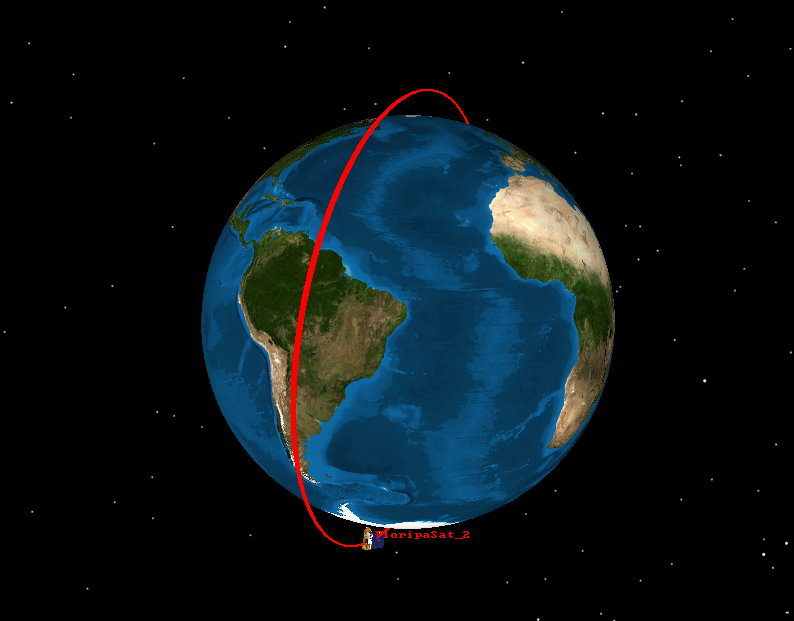
\includegraphics[width=0.6\textwidth]{figures/fsat2-gmat.png}
        \caption{GOLDS-UFSC orbit simulation on GMAT.}
        \label{fig:fsat2-gmat}
    \end{center}
\end{figure}

\begin{figure}[!ht]
    \begin{center}
        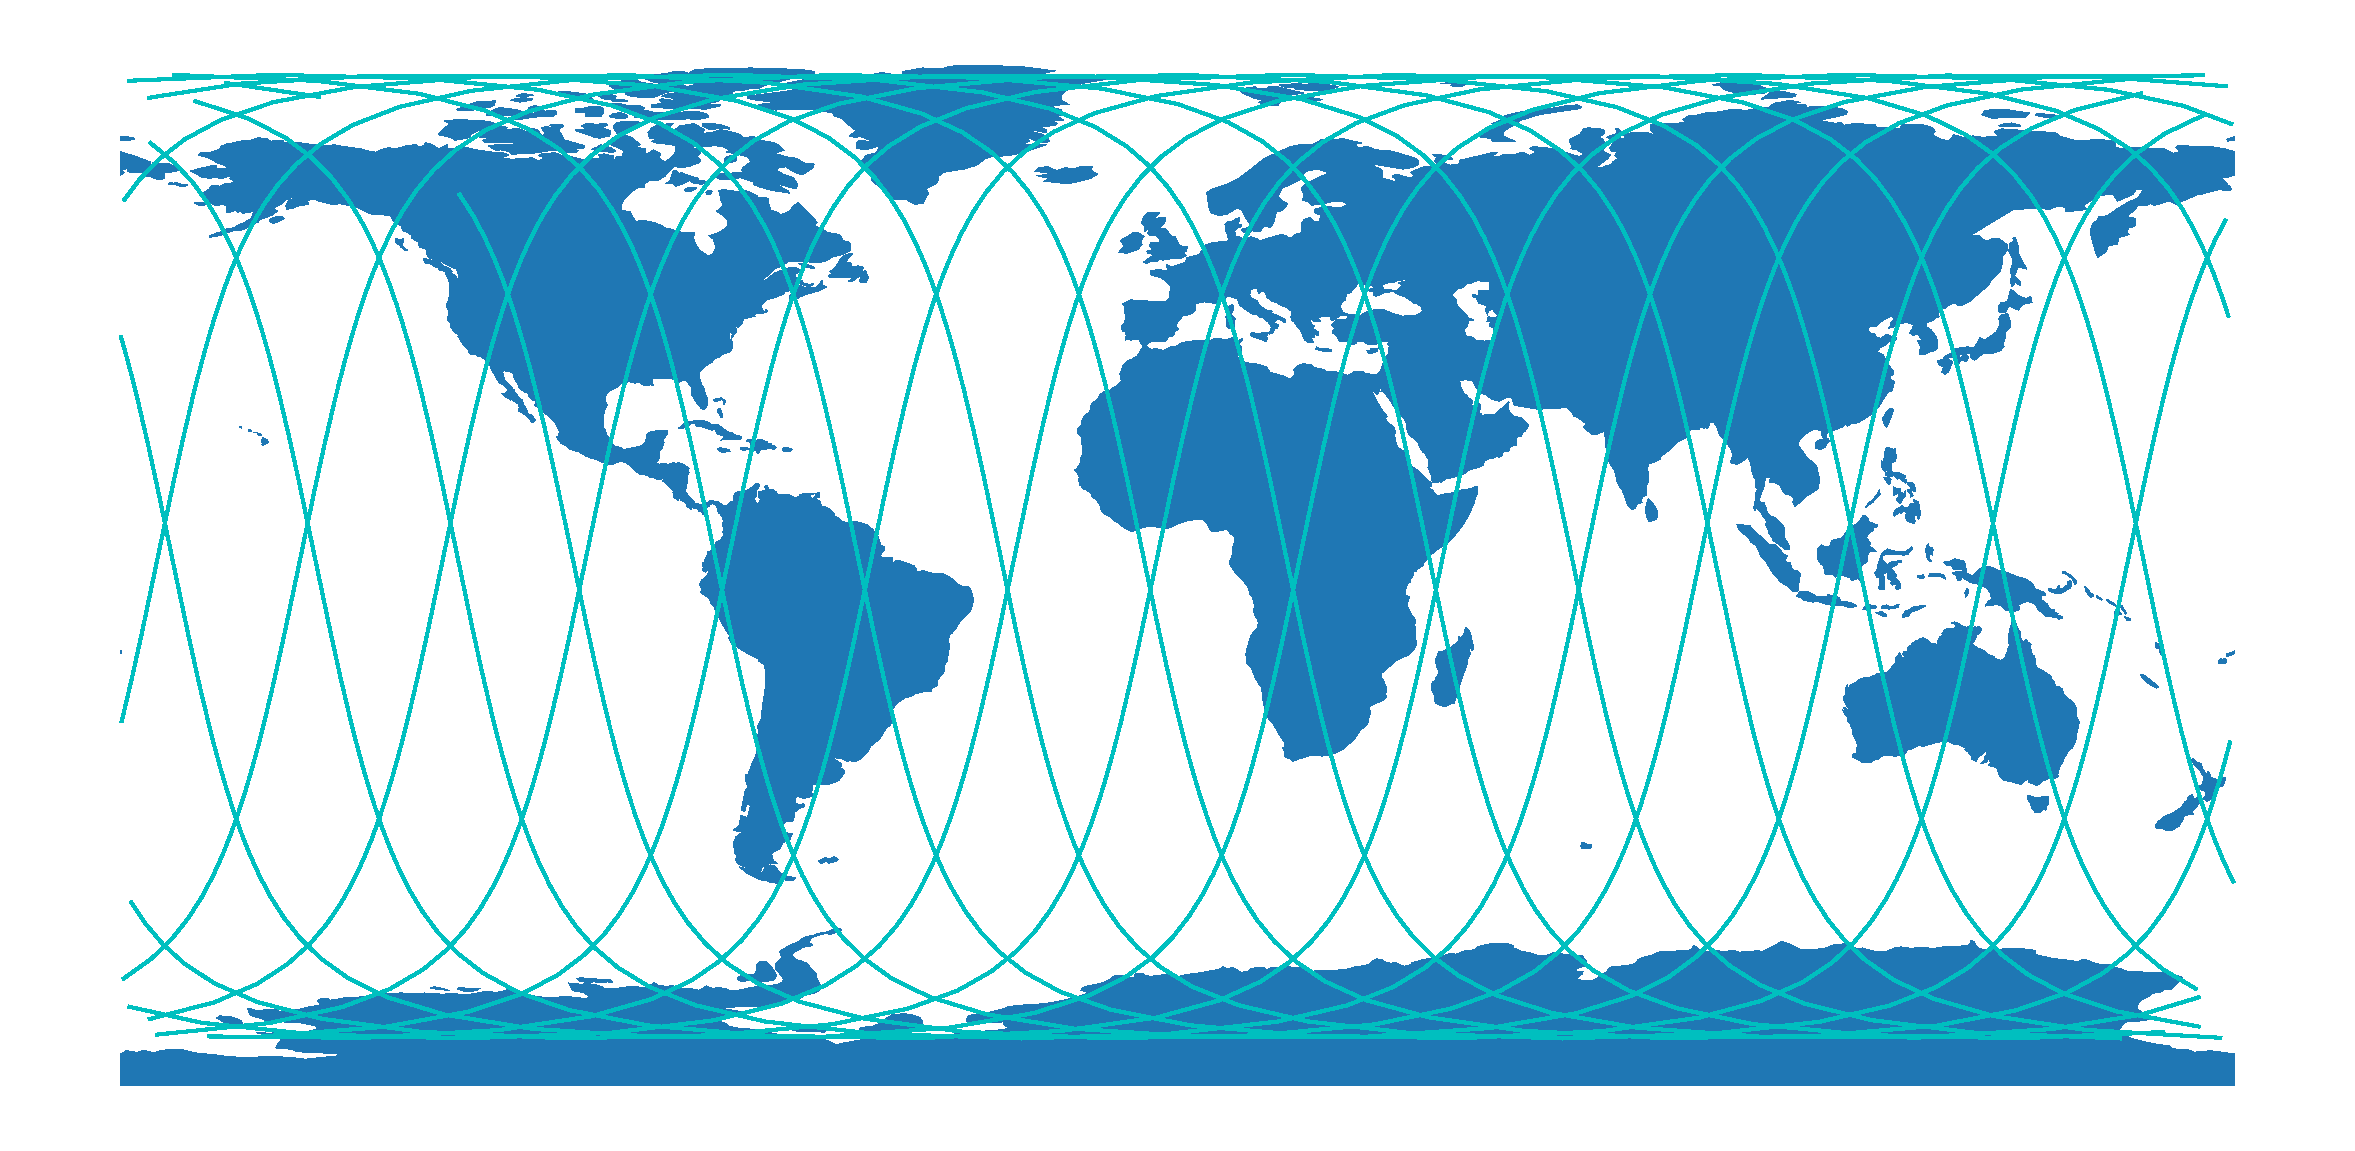
\includegraphics[width=\textwidth]{figures/fsat2-gmat-groundtrack.pdf}
        \caption{GOLDS-UFSC simulated groundtrack.}
        \label{fig:fsat2-gmat-groundtrack}
    \end{center}
\end{figure}

The next sections present some analysis based on the results obtained from the simulations performed with SimCube.% executed on GMAT.

%The source files of the GMAT simulation are available in \cite{fsat2-mechanical}.

\subsection{Lifetime Analysis}

Considering the same parameters of FloripaSat-1, but with an initial altitude of 550 km, the simulations on SimCube showed that the satellite decays approximately in 2183 days ($\cong$ 6 years), as can be seen in \autoref{fig:lifetime-analysis}.

\begin{figure}[!ht]
    \begin{center}
        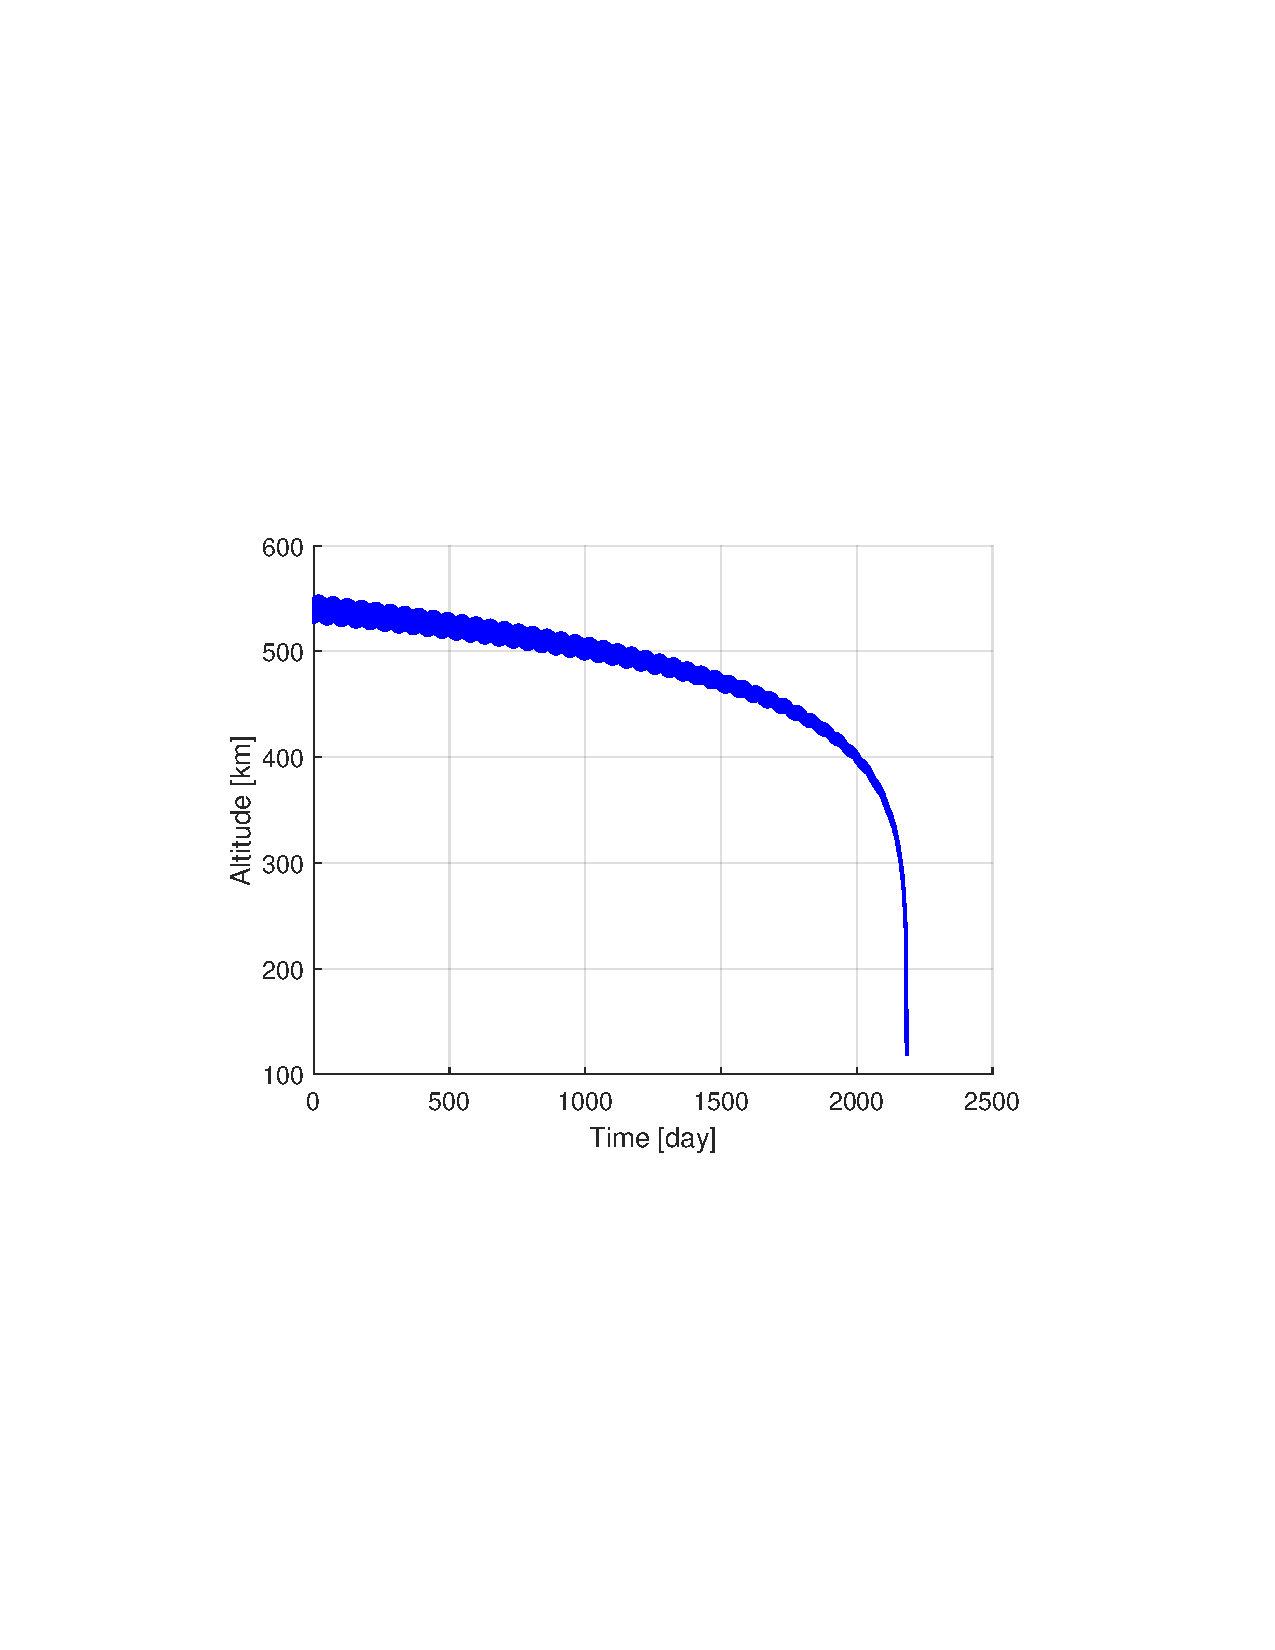
\includegraphics[trim=3.5cm 8cm 4.0cm 8cm,clip, width=0.8\textwidth]{curves/Altitude.pdf}
        \caption{Lifetime analysis.}
        \label{fig:lifetime-analysis}
    \end{center}
\end{figure}

\subsection{Ground Station Passes and Data Transfer Analysis}

Considering two ground stations, one at the SpaceLab installations in Florianópolis (27$^{\circ}$ 36' 00.9" S, 48$^{\circ}$ 31' 03.2" W) and other at the INPE/CRN installations in Natal (5$^{\circ}$ 50' 10.1" S, 35$^{\circ}$ 12' 27.5" W), both with a minimum elevation of 15$^{\circ}$, the results in \autoref{tab:grs-contacts-analysis}) were achieved. %during the simulations on GMAT .

\begin{table}[!ht]
    \centering
    \begin{tabular}{lccc}
        \toprule[1.5pt]
        \textbf{Parameter} & \textbf{UFSC Station} & \textbf{INPE-RN Station} & \textbf{Unit} \\
        \midrule
        Minimum elevation to a valid contact    & 15    & 15    & $^{\circ}$ \\
        Number of contacts                      & 143   & 125   & - \\
        Minimum contract period                  & 24    & 34    & sec \\
        Maximum contact period                  & 395   & 394   & sec \\
        Average contact period                  & 303   & 298   & sec \\
        Total contact period                    & 43394 & 37205 & sec \\
        \bottomrule[1.5pt]
    \end{tabular}
    \caption{Ground station contacts analysis during the first 60 days of operation.}
    \label{tab:grs-contacts-analysis}
\end{table}

As seen from \autoref{tab:grs-contacts-analysis}, during the first 60 days of operation, considering the two main ground stations that will contact the satellite, the total contact period is 80599 seconds (43394 + 37205). With the data rate of the downlink/uplink as 4800 bps, this period will allow a data transfer of 48359400 bytes (or 46.12 M$_{i}$B) between GOLDS-UFSC and the Earth. Using the satellite's lifetime from the previous analysis (2000 days), and an average data transfer per day of 805990 bits, the total theoretical raw data transfer during the whole operation of the satellite will be approximately 1.5 G$_{i}$B.

These values can be even more significant if a smaller minimum elevation is considered, or with more ground stations in other locations.

\section{Mass Budget} \label{mass-budget}

The mass budget of the satellite can be seen in \autoref{tab:mass-budget}.

\begin{table}[!ht]
    \centering
    \begin{tabular}{llc}
        \toprule[1.5pt]
        \textbf{Subsystem} & \textbf{Model} & \textbf{Mass [g]} \\
        \midrule
        OBDH                        & SpaceLab OBDH 2.0             & 53 \\
        TTC                         & SpaceLab TTC 2.0              & 52 \\
        EPS                         & SpaceLab EPS 2.0              & 80 \\
        Battery                     & SpaceLab Battery Module 4C    & 235 \\
        Antenna TTC                 & ISISpace AntS                 & 89 \\
        ACS                         & SpaceLab Passive ACS 2U       & 100 (TBC) \\
        Payload 1                   & INPE-RN EDC                   & 75 \\
        Payload 2                   & SpaceLab ExpLoRa              & \textcolor{red}{TBD} \\
        Antenna Payloads            & ISISpace AntS                 & 89 \\
        Interface                   & SpaceLab Interface Boards     & 40 \\
        PC-104 Adapter              & SpaceLab PC-104 Adapter       & 50 (TBC) \\
        Solar Panel                 & Orbital Custom Solar Panel    & 266 \\
        Shields                     & 3 mm aluminum sheets          & 590 (TBC) \\
        Structure                   & Usiped Custom 2U Structure    & 206 \\
        Cables                      & -                             & 200 \\
        Others                      & -                             & 100 \\
        \midrule
        Total                       & -                             & \textbf{2277} \\
        Max. CubeSat 2U             & -                             & 2666 \\
        Margin                      & -                             & 389 \\
        \bottomrule[1.5pt]
    \end{tabular}
    \caption{Mass budget of the satellite.}
    \label{tab:mass-budget}
\end{table}

According to the CubeSat standard \cite{cds}, the maximum mass of each unit must be 1.33 kg. As the GOLDS-UFSC is a 2U CubeSat, the maximum allowed mass of the project is 2.66 kg. Considering the weight of each subsystem presented in \autoref{tab:mass-budget}, the current total mass of the object is below the maximum allowed, with a margin of 15 \%.

\section{Power Budget} \label{power-budget}

According to section 10.3 of \cite{larson2005}, the power budget of a satellite can be determined through three steps:

\begin{enumerate}
    \item Prepare operating power budget
    \item Size the battery
    \item Estimate power degradation over mission life
\end{enumerate}

\subsection{Input Power}

Simulations of the energy input to the solar panels along some orbits can be seen in the \autoref{fig:sp_sim_power} graph. Two extreme orbit scenarios, without and with maximum eclipse, were tested. The figures show the power generated on each side of the CubeSat, as well the total and average values.

\begin{figure}[!ht]
    \begin{center}
        \subfloat[Maximum eclipse.]{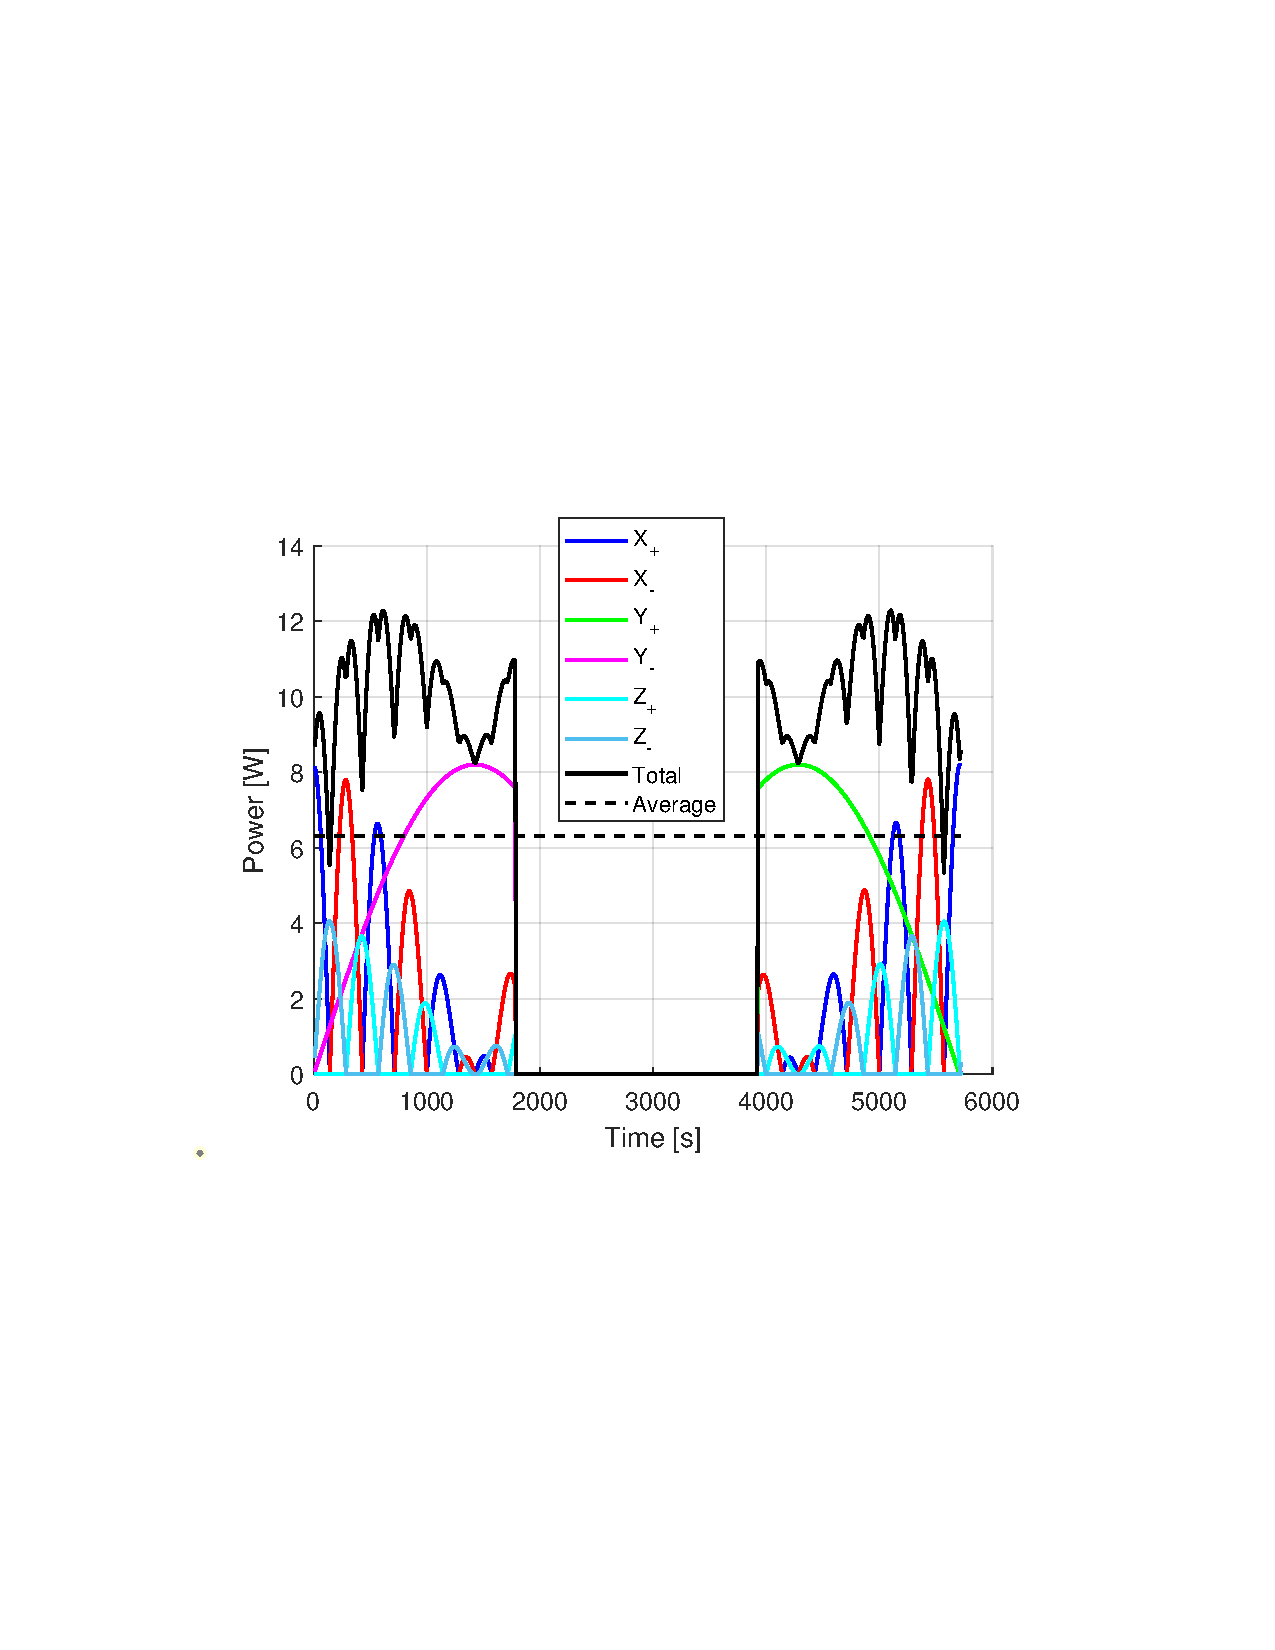
\includegraphics[width=0.45\columnwidth]{curves/GOLDS_com_eclipse.pdf}}
        ~
        \subfloat[Without eclipse.\label{fig:without_eclipse}]
        {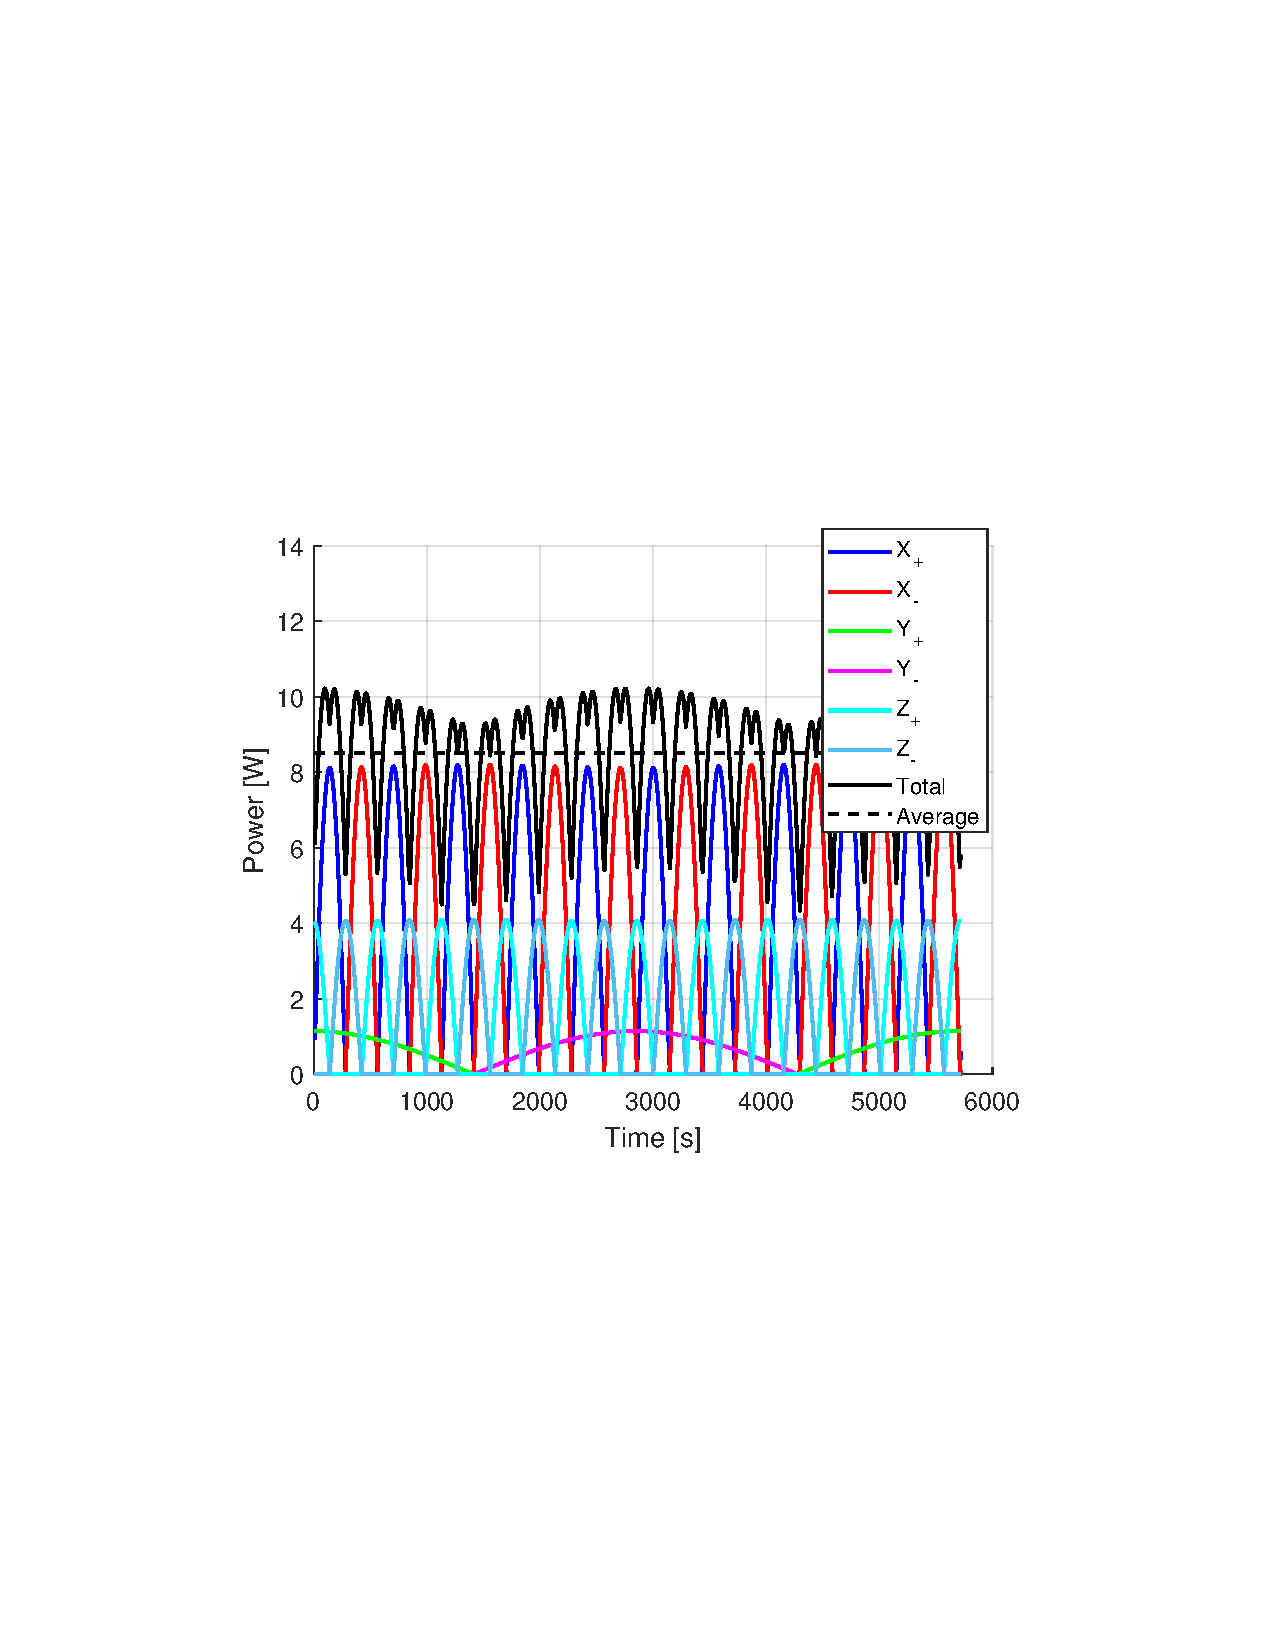
\includegraphics[trim=4cm 8.5cm 4cm 8.5cm, clip, width=0.45\textwidth]{curves/GOLDS_sem_eclipse.pdf}}
        \caption{Simulated input power of the solar panels.}
        \label{fig:sp_sim_power}
    \end{center}
\end{figure}

From these simulations, the results in \autoref{tab:power-simulations} were obtained:

\begin{table}[!ht]
    \centering
    \begin{tabular}{lcc}
        \toprule[1.5pt]
        \textbf{Parameter} & \textbf{Maximum eclipse} & \textbf{Without eclipse} \\    \midrule
        Peak power & 12282.7 mW & 10217.2 mW\\
        Average power (total orbit) & 6306.9 mW & 8519.6 mW \\
        Average (sunlight) & 10048.9 mW & 8519.6 mW\\
        Orbit period & 5720 s & 5720 s \\
        Sun light period &  3590 s & 5720 s\\
        Eclipse period & 2130 s & 0 s \\
        \bottomrule[1.5pt]
    \end{tabular}
    \caption{Results for the power input.}
    \label{tab:power-simulations}
\end{table}


\subsection{Operating Power Budget}

Typical operating voltages and current and power ranges consumed by each satellite subsystem are presented in \autoref{tab:power-requirements}.

\begin{table}[!ht]
    \centering
    \begin{tabular}{lccccc}
        \toprule[1.5pt]
        \multirow{2}{*}{\textbf{Module}} & \multirow{2}{*}{\textbf{Voltage [V]}}    & \multicolumn{2}{c}{\textbf{Current [mA]}} & \multicolumn{2}{c}{\textbf{Power [mW]}} \\
                                         &                                          & \textbf{Min.} & \textbf{Max.}             & \textbf{Min.} & \textbf{Max.} \\
        \midrule
        OBDH                & 3.3   & 35    & 200   & 115   & 660 \\
        TTC ($\mu$C)        & 3.3   & 40    & 40    & 132   & 132 \\
        TTC (radio module)  & 5     & 10    & 650   & 33    & 3250 \\
        EPS (digital part)  & 7.4   & 50    & 260   & 165   & 858 \\
        EPS (heater)        & 7.4   & 675   & 675   & 5000  & 5000 \\
        Antenna module      & 3.3   & 60    & 550   & 200   & 1800 \\
        Payload EDC         & 5     & 250   & 250   & 1250  & 1250 \\
        Radiation instrument           & 5     & TBD   & TBD   & TBD   & TBD \\
        \bottomrule[1.5pt]
    \end{tabular}
    \caption{Power requirements of the subsystems and payloads of the satellite.}
    \label{tab:power-requirements}
\end{table}

Using the information presented in \autoref{tab:power-requirements}, and the activation periods defined for each module (the duty cycle), we arrive at the average satellite consumption present in \autoref{tab:power-consumption}.

\begin{table}[!ht]
    \centering
    \begin{tabular}{lccccc}
        \toprule[1.5pt]
        \textbf{Module} & \textbf{Duty Cycle [\%]}    & \textbf{Power [mW]} \\
        \midrule
        OBDH                    & 100   & 115 \\
        TTC (radio 1 RX)        & 95    & 65 \\
        TTC (radio 1 TX)        & 5     & 3250 \\
        TTC (radio 2 RX)        & 95    & 65 \\
        TTC (radio 2 TX)        & 5     & 3250 \\
        EPS                     & 100   & 320 \\
        BAT (idle)              & 90    & 0 \\
        BAT (heater full)       & 10    & 5000 \\
        Antenna (deployment)    & 0     & 1800 \\
        Antenna (deployed)      & 100   & 35 \\
        Payload EDC             & 100   & 1250 \\
        Radiation instrument        & 0     & 1000 \\
        \cmidrule{2-3}
        Satellite               & \multicolumn{2}{c}{$\cong$ 2668} \\
        \bottomrule[1.5pt]
    \end{tabular}
    \caption{Power consumption of the subsystems and payloads of the satellite.}
    \label{tab:power-consumption}
\end{table}

The duty cycles of \autoref{tab:power-consumption} were defined according to the following assumptions:

\begin{itemize}
    \item One of the EDC payload is always off (cold redundancy).
    \item The Radiation instrument is turned on just during limited periods and only with telecommands.
\end{itemize}

As can be seen from \autoref{fig:sp_sim_power} and \autoref{tab:power-consumption}, there is a slight positive margin of \textbf{76.9 mW} in the power budget.

\subsection{Battery Sizing}

As described in \cite{larson2005}, the battery sizing of a satellite can be made by following the steps below:

\begin{enumerate}
    \item Estimate power level that the battery must supply
    \item Compute discharge cycle duration, charge cycle duration, and numbers of charge-discharge cycles
    \item Select depth of discharge
    \item Select charge rate
    \item Compute battery recharge power
\end{enumerate}

The power level that the battery must supply is the total power consumption of the satellite and is available in \autoref{tab:power-consumption}.

The discharge and charge cycle duration can be obtained from \autoref{fig:sp_sim_power}. The discharge duration is approximately 35.3 min (or 0.5889 h), and the charge cycle duration is 61.83 min (or 1.031 h). This is considering a single complete orbit.

The depth of discharge (DoD) can be obtained using the \autoref{eq:dod-equation}.

\begin{equation} \label{eq:dod-equation}
    DoD = \frac{D_{i} \cdot D_{t}}{C} \cdot 100\ \%
\end{equation}

Where:

\begin{itemize}
    \item $D_{i}$: Discharge rate
    \item $D_{t}$: Discharge period
    \item $C$: Battery capacity
\end{itemize}

As the battery cells are already selected (5000 mAh in total, as described in \autoref{ssec:battery-module}), the current DoD is computed in \autoref{eq:dod-value}.

\begin{equation} \label{eq:dod-value}
    DoD = \frac{2668\ mW \cdot 0.5889\ h}{18500\ mWh} \cdot 100 \cong \mathbf{8.5\ \%}
\end{equation}

The charge rate can be estimated from the power input of the solar panels when the satellite is in sunlight. As presented before, the simulation results estimate the power input as 4315.6 mW. Considering the charge time as 61.83 min (or 1.031 h), the input energy is 4450 mWh. From \autoref{tab:power-consumption}, the power consumption of the satellite at sunlight is 2169 mW (or 2236 mWh considering the sunlight period). This way, energy input at sunlight is obtained in \autoref{eq:energy-input-sun-light}.

\begin{equation} \label{eq:energy-input-sun-light}
    4450 - 2236 = 2214\ mWh
\end{equation}

From the DoD calculation, the energy consumption during the eclipse is 1571 mWh. This way, the energy margin of the battery becomes positive ($2214 - 1571 = 643 mWh$), as expected from the power budget results.

All results from the battery sizing are available in \autoref{tab:battery-sizing-results}.

\begin{table}[!ht]
    \centering
    \begin{tabular}{lcc}
        \toprule[1.5pt]
        \textbf{Parameter} & \textbf{Value}    & \textbf{Unit} \\
        \midrule
        Battery capacity                & 18500  & mWh \\
        Energy consumption on sunlight & 2169   & mWh \\
        Energy consumption on eclipse   & 1571   & mWh \\
        Sunlight duration              & 1.031  & h \\
        Eclipse duration                & 0.5889 & h \\
        Depth of Discharge (DoD)        & 8.5    & \% \\
        Total battery energy margin     & 643    & mWh \\
        \bottomrule[1.5pt]
    \end{tabular}
    \caption{Battery sizing results.}
    \label{tab:battery-sizing-results}
\end{table}

From the results, the battery sizing is well suited for the current satellite configuration and the planned behavior.

\subsection{Power Degradation Over Mission Life}

Two major events along the satellite operation should be considered in the power degradation analysis:

\begin{enumerate}
    \item Solar panels degradation
    \item Battery degradation
\end{enumerate}

From \cite{larson2005}, 5 \% per year is a usual number for the solar panels' degradation, in other words, the general efficiency of the solar panels decays at a rate of 5 \% per year of operation.% Also, \cite{larson2005} defines the battery degradation (or aging )as XX \% per year.

%A partial discharge reduces stress and prolongs battery life, so does a partial charge. Elevated temperature and high currents also affect cycle life

\section{Link Budget}

The link budget of all satellite radio links is available in \autoref{tab:link-budget-results}.

\begin{table}[!ht]
    \centering
    \begin{tabular}{L{0.3\textwidth}cccc}
        \toprule[1.5pt]
        \textbf{Variable} & \textbf{Downlink} & \textbf{Uplink} & \textbf{Uplink (Payload)} & \textbf{Unit}\\
        \midrule
        Altitude                        & 550           & 550           & 550           & km \\
        Elevation                       & 0             & 0             & 0             & $^{\circ}$ \\
        Frequency                       & 468           & 401           & 401.635       & MHz \\
        Modulation                      & GMSK          & GMSK          & BPSK          & - \\
        Protocol                        & NGHam         & NGHam         & SBCD          & - \\
        Transmit power                  & 30            & 44            & 30            & dBm \\
        Transmitter antenna gain        & 0             & 12            & 3             & dBi \\
        Receiver antenna gain           & 12            & 0             & 0             & dBi \\
        FSPL                            &               &               & 153.2         & dB \\
        Power at receiver               &               &               & -125.2        & dBm \\
        Receiver sensibility            & -134          & -126          & -128          & dBm \\
        System losses                   & 5             & 5             & 5             & dB \\
        Receiver noise temp.            &               &               & 361.7         & K \\
        Antenna noise temp.             & 300           & 300           & 300           & K \\
        System noise temp.              &               &               & 661.7         & K \\
        Data rate                       & 4800          & 4800          & 400           & bps \\
        Received SNR                    &               &               & 19.17         & dB \\
        SNR required for $10^{-5}$ BER\footnotemark & 9.6           & 9.6           & 9.6           & dB \\
        Link margin                     &               &               & $\geq$ 9.57   & dB \\
        \bottomrule[1.5pt]
    \end{tabular}
    \caption{Link budget results.}
    \label{tab:link-budget-results}
\end{table}

\footnotetext{Without FEC.}

As can be seen, considering the worst case for the estimated orbit, that is, with the satellite on the horizon and with an elevation of zero degrees, the margin of all links is positive with a considerable balance.

All equations and steps used to obtain the results of \autoref{tab:link-budget-results} are available in \autoref{anx:link-budget}.
